\section{Derivada Direccional y Vector Gradiente}

Las derivadas parciales $f_x$ y $f_y$ miden la tasa de cambio de $f$ en las direcciones de los ejes coordenados. La derivada direccional generaliza esta idea a una dirección arbitraria en el plano.

\subsection{Derivada direccional}

Sea $\mathbf{u} = \langle u_1, u_2 \rangle$ un vector unitario en $\mathbb{R}^2$ y sea $(x_0, y_0)$ un punto en el dominio de $f$. La tasa de cambio de $f$ en la dirección de $\mathbf{u}$ se obtiene restringiendo $f$ a la recta que pasa por $(x_0, y_0)$ con dirección $\mathbf{u}$:
\[
\mathbf{r}(h) = (x_0 + hu_1,\; y_0 + hu_2), \qquad h \in \mathbb{R}.
\]

\begin{mydefinition}{Derivada direccional}
Sea $f: D \subseteq \mathbb{R}^2 \to \mathbb{R}$ y sea $\mathbf{u} = \langle u_1, u_2 \rangle$ un vector unitario. La derivada direccional de $f$ en $(x_0, y_0)$ en la dirección de $\mathbf{u}$ es:
\[
D_{\mathbf{u}} f(x_0, y_0)
= \lim_{h \to 0} \frac{f(x_0 + hu_1,\, y_0 + hu_2) - f(x_0, y_0)}{h}
\]
siempre que el límite exista.
\end{mydefinition}

Geométricamente, el plano vertical que pasa por $(x_0, y_0, 0)$ en la dirección de $\mathbf{u}$ corta a la superficie $z = f(x,y)$ en una curva $C$. La derivada direccional $D_{\mathbf{u}} f(x_0, y_0)$ es la pendiente de la recta tangente a $C$ en $P_0$.

Si $\mathbf{u} = \mathbf{i} = \langle 1, 0 \rangle$, la definición reproduce $f_x(x_0, y_0)$; si $\mathbf{u} = \mathbf{j} = \langle 0, 1 \rangle$, reproduce $f_y(x_0, y_0)$. Las derivadas parciales son casos particulares de la derivada direccional.

Calcular derivadas direccionales mediante la definición límite es trabajoso. Cuando $f$ es diferenciable, la regla de la cadena proporciona una fórmula algebraica directa.

\begin{mytheorem}{Fórmula de la derivada direccional}
Si $f$ es diferenciable en $(x_0, y_0)$ y $\mathbf{u} = \langle u_1, u_2 \rangle$ es unitario, entonces:
\[
D_{\mathbf{u}} f(x_0, y_0) = f_x(x_0, y_0)\, u_1 + f_y(x_0, y_0)\, u_2
\]
\end{mytheorem}

\textit{Demostración.} La idea es reconocer que el cociente de la definición es, en realidad, la derivada de una función de una sola variable, a la cual se le puede aplicar la regla de la cadena ya estudiada.

Se restringe $f$ a la recta que pasa por $(x_0, y_0)$ con dirección $\mathbf{u}$, definiendo:
\[
g(h) = f\bigl(x(h),\, y(h)\bigr), \qquad x(h) = x_0 + hu_1, \quad y(h) = y_0 + hu_2.
\]
Con esta notación, el cociente incremental de la definición es precisamente el cociente incremental de $g$ en $h = 0$:
\[
\frac{f(x_0 + hu_1,\, y_0 + hu_2) - f(x_0, y_0)}{h}
= \frac{g(h) - g(0)}{h}.
\]
Tomando el límite cuando $h \to 0$, el lado derecho es por definición la derivada $g'(0)$, de modo que:
\[
D_{\mathbf{u}} f(x_0, y_0) = g'(0).
\]
Ahora bien, $g$ es la composición de $f$ con las funciones $x(h)$ e $y(h)$, así que su derivada se obtiene con la regla de la cadena para $z = f(x, y)$ donde $x$ e $y$ dependen de una variable $h$:
\[
g'(h) = \frac{dz}{dh}
= \frac{\partial f}{\partial x}\,\frac{dx}{dh} + \frac{\partial f}{\partial y}\,\frac{dy}{dh}.
\]
Las derivadas de las componentes son constantes, pues $x(h)$ e $y(h)$ son lineales en $h$:
\[
\frac{dx}{dh} = u_1, \qquad \frac{dy}{dh} = u_2.
\]
Sustituyendo:
\[
g'(h) = f_x\bigl(x(h), y(h)\bigr)\,u_1 + f_y\bigl(x(h), y(h)\bigr)\,u_2.
\]
Al evaluar en $h = 0$ se tiene $x(0) = x_0$ e $y(0) = y_0$, con lo que las parciales se calculan en el punto original:
\[
D_{\mathbf{u}} f(x_0, y_0) = g'(0) = f_x(x_0, y_0)\,u_1 + f_y(x_0, y_0)\,u_2.
\]
Esto explica por qué la definición límite, que en principio no menciona las derivadas parciales, produce un resultado expresado en términos de ellas: al restringir $f$ a la recta de dirección $\mathbf{u}$, la regla de la cadena descompone la tasa de cambio en las contribuciones de cada variable, $f_x$ y $f_y$, ponderadas por las componentes $u_1$ y $u_2$ de la dirección. $\square$

\textbf{Ejemplo.} Sea $f(x, y) = x^2 y + \sin(xy)$ y $\mathbf{u}$ la dirección del ángulo $\theta = \pi/3$, es decir $\mathbf{u} = \langle 1/2,\, \sqrt{3}/2 \rangle$. En el punto $(1, 0)$:
\[
f_x = 2xy + y\cos(xy)\big|_{(1,0)} = 0, \qquad f_y = x^2 + x\cos(xy)\big|_{(1,0)} = 2.
\]
Luego $D_{\mathbf{u}} f(1, 0) = 0 \cdot \tfrac{1}{2} + 2 \cdot \tfrac{\sqrt{3}}{2} = \sqrt{3}$.

\subsection{Vector gradiente}

La fórmula $D_{\mathbf{u}} f = f_x u_1 + f_y u_2$ es el producto punto de $\langle f_x, f_y \rangle$ con $\mathbf{u}$. El vector $\langle f_x, f_y \rangle$ reúne toda la información de primer orden de $f$ y recibe el nombre de gradiente.

\begin{mydefinition}{Vector gradiente}
Sea $f: D \subseteq \mathbb{R}^2 \to \mathbb{R}$ diferenciable. El gradiente de $f$ en $(x, y)$ es el vector:
\[
\nabla f(x, y) = \langle f_x(x, y),\; f_y(x, y) \rangle = f_x\,\mathbf{i} + f_y\,\mathbf{j}
\]
La derivada direccional se expresa entonces como:
\[
D_{\mathbf{u}} f(x_0, y_0) = \nabla f(x_0, y_0) \cdot \mathbf{u}
\]
\end{mydefinition}

El gradiente es un campo vectorial: asigna a cada punto del dominio un vector en $\mathbb{R}^2$. Su valor en un punto resume la pendiente de $f$ en todas las direcciones simultáneamente.

\textbf{Ejemplo.} Para $f(x, y) = x^2 - xy + y^3$, el gradiente es $\nabla f = \langle 2x - y,\; -x + 3y^2 \rangle$. En el punto $(2, 1)$: $\nabla f(2,1) = \langle 3,\; 1 \rangle$.

La derivada direccional en la dirección de $\mathbf{v} = \langle 3, 4 \rangle$ (que se normaliza a $\mathbf{u} = \langle 3/5, 4/5 \rangle$) es:
\[
D_{\mathbf{u}} f(2,1) = \langle 3, 1 \rangle \cdot \langle \tfrac{3}{5}, \tfrac{4}{5} \rangle = \frac{9}{5} + \frac{4}{5} = \frac{13}{5}.
\]

\subsection{Generalización para $n$ variables}

La extensión al caso de $n$ variables es inmediata: se reemplaza $\mathbb{R}^2$ por $\mathbb{R}^n$ y el vector unitario se toma en $\mathbb{R}^n$.

\begin{mydefinition}{Derivada direccional en $\mathbb{R}^n$}
Sea $f: D \subseteq \mathbb{R}^n \to \mathbb{R}$ y $\mathbf{u} \in \mathbb{R}^n$ con $\|\mathbf{u}\| = 1$. La derivada direccional de $f$ en $\mathbf{x}_0$ en la dirección $\mathbf{u}$ es:
\[
D_{\mathbf{u}} f(\mathbf{x}_0) = \lim_{h \to 0} \frac{f(\mathbf{x}_0 + h\mathbf{u}) - f(\mathbf{x}_0)}{h}
\]
Si $f$ es diferenciable, $D_{\mathbf{u}} f(\mathbf{x}_0) = \nabla f(\mathbf{x}_0) \cdot \mathbf{u}$, donde el gradiente es:
\[
\nabla f(\mathbf{x}_0) = \left\langle \frac{\partial f}{\partial x_1}(\mathbf{x}_0),\; \dots,\; \frac{\partial f}{\partial x_n}(\mathbf{x}_0) \right\rangle
\]
\end{mydefinition}

\textbf{Ejemplo.} Sea $f(x, y, z) = x^2 + y^2 + z^2$. El gradiente es $\nabla f = \langle 2x, 2y, 2z \rangle = 2\mathbf{r}$, proporcional al vector posición. En el punto $(1, 1, 1)$ y con $\mathbf{u} = \langle 1, 1, 1 \rangle / \sqrt{3}$:
\[
D_{\mathbf{u}} f(1,1,1) = \langle 2, 2, 2 \rangle \cdot \frac{\langle 1,1,1\rangle}{\sqrt{3}} = \frac{6}{\sqrt{3}} = 2\sqrt{3}.
\]

\subsection{Maximización de la derivada direccional}

La expresión $D_{\mathbf{u}} f = \nabla f \cdot \mathbf{u} = \|\nabla f\|\,\|\mathbf{u}\|\cos\phi = \|\nabla f\|\cos\phi$, donde $\phi$ es el ángulo entre $\nabla f$ y $\mathbf{u}$, permite determinar las direcciones extremas.

\begin{mytheorem}{Dirección de máximo y mínimo crecimiento}
Sea $f$ diferenciable en $\mathbf{x}_0$ con $\nabla f(\mathbf{x}_0) \neq \mathbf{0}$. Entonces:
\begin{itemize}
    \item $D_{\mathbf{u}} f(\mathbf{x}_0)$ es máxima cuando $\mathbf{u} = \dfrac{\nabla f(\mathbf{x}_0)}{\|\nabla f(\mathbf{x}_0)\|}$, y el valor máximo es $\|\nabla f(\mathbf{x}_0)\|$.
    \item $D_{\mathbf{u}} f(\mathbf{x}_0)$ es mínima cuando $\mathbf{u} = -\dfrac{\nabla f(\mathbf{x}_0)}{\|\nabla f(\mathbf{x}_0)\|}$, y el valor mínimo es $-\|\nabla f(\mathbf{x}_0)\|$.
    \item $D_{\mathbf{u}} f(\mathbf{x}_0) = 0$ cuando $\mathbf{u} \perp \nabla f(\mathbf{x}_0)$.
\end{itemize}
\end{mytheorem}

El tercer punto tiene una consecuencia geométrica importante: el gradiente es perpendicular a las curvas de nivel de $f$. En efecto, si $f(x,y) = c$ define una curva y $\mathbf{r}(t)$ la parametriza, entonces $\frac{d}{dt}f(\mathbf{r}(t)) = \nabla f \cdot \mathbf{r}'(t) = 0$, con lo que $\nabla f$ es normal a $\mathbf{r}'(t)$, que es el vector tangente a la curva de nivel.

\begin{center}
\shorthandoff{>}
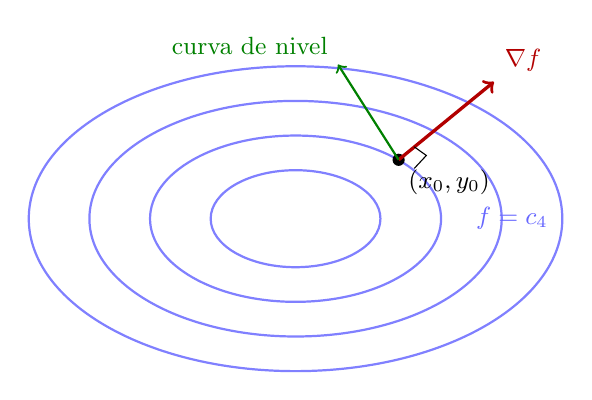
\begin{tikzpicture}[scale=1.1, every node/.style={font=\small}]
    % Curvas de nivel (elipses)
    \foreach \r in {0.7, 1.2, 1.7, 2.2} {
        \draw[blue!50, thick] (0,0) ellipse ({\r*1.4} and {\r*0.8});
    }
    % Punto base
    \fill (1.4*0.85, 0.8*0.85) circle (2pt) node[below right] {$(x_0, y_0)$};
    % Gradiente
    \draw[->, very thick, red!70!black]
        (1.4*0.85, 0.8*0.85) -- ++(1.1, 0.9)
        node[above right] {$\nabla f$};
    % Dirección de una curva de nivel (tangente)
    \draw[->, thick, green!50!black]
        (1.4*0.85, 0.8*0.85) -- ++(-0.7, 1.1)
        node[above left] {curva de nivel};
    % Ángulo recto
    \draw (1.4*0.85+0.18, 0.8*0.85+0.15) -- ++(0.14, -0.10) -- ++(-0.14, -0.15);
    % Etiquetas de nivel
    \node[blue!60] at (2.5, 0) {$f = c_4$};
\end{tikzpicture}
\end{center}

El gradiente en $(x_0, y_0)$ apunta en la dirección de máximo crecimiento de $f$ y es perpendicular a la curva de nivel que pasa por ese punto.

\textbf{Ejemplo.} Sea $f(x, y) = 4x^2 + y^2$. En el punto $(1, 2)$: $\nabla f(1, 2) = \langle 8, 4 \rangle$. El máximo crecimiento es $\|\nabla f\| = \sqrt{64 + 16} = 4\sqrt{5}$, y ocurre en la dirección $\mathbf{u} = \langle 8, 4 \rangle / (4\sqrt{5}) = \langle 2, 1 \rangle / \sqrt{5}$.

\subsection{Ejercicios}
\begin{enumerate}
    \item Calcule la derivada direccional de las siguientes funciones en el punto y dirección indicados usando la definición límite, y verifique el resultado con la fórmula del gradiente.
\begin{enumerate}
    \item $f(x, y) = 3x^2 - 2xy + y^2$ en $(1, 2)$, dirección $\mathbf{u} = \langle 1/\sqrt{2},\, 1/\sqrt{2} \rangle$.
    \item $f(x, y) = x^2 + xy$ en $(0, 1)$, dirección $\mathbf{u} = \langle 3/5,\, 4/5 \rangle$.
\end{enumerate}

    \item Calcule el gradiente de cada función y evalúelo en el punto dado.
\begin{enumerate}
    \item $f(x, y) = \ln(x^2 + y^2)$ en $(1, 2)$.
    \item $f(x, y) = e^{x}\sin(y)$ en $(0, \pi/6)$.
    \item $f(x, y) = \arctan(y/x)$ en $(1, 1)$.
\end{enumerate}

    \item Sea $f(x, y) = \sqrt{4 - x^2 - 2y^2}$.
\begin{enumerate}
    \item Calcule $\nabla f(1, 1)$.
    \item Encuentre la derivada direccional en $(1, 1)$ en la dirección del punto $(1, 1)$ al punto $(3, 2)$.
    \item Determine la dirección en que $f$ decrece con mayor rapidez en $(1, 1)$ y calcule esa tasa de decrecimiento.
\end{enumerate}

    \item La temperatura en una placa metálica está dada por $T(x, y) = 100 - 3x^2 - 5y^2$ (en $^\circ$C), con $x$ e $y$ en metros.
\begin{enumerate}
    \item Encuentre el gradiente de $T$ en el punto $(1, 2)$.
    \item En ese punto, ¿en qué dirección debe moverse un punto de la placa para que la temperatura suba con mayor rapidez? ¿Cuál es esa tasa máxima de cambio?
    \item Calcule la derivada direccional en la dirección que forma $\pi/4$ con el eje $x$.
\end{enumerate}

    \item Calcule la derivada direccional de $f(x, y, z) = x^2 y + y^2 z + z^2 x$ en el punto $(1, 1, 1)$ en la dirección del vector $\mathbf{v} = \langle 2, -1, 2 \rangle$. Encuentre además la tasa máxima de cambio de $f$ en ese punto.

    \item Encuentre todos los puntos del dominio en los que el gradiente de $f(x, y) = x^3 - 3xy + y^3$ es el vector cero. Clasifique esos puntos como posibles máximos, mínimos o puntos de silla a partir de la información que proporciona el gradiente (sin usar el criterio de la segunda derivada).

    \item Demuestre que el gradiente de $f(x, y)$ es perpendicular a la curva de nivel $f(x, y) = c$ en cualquier punto de la curva. Use este resultado para encontrar la ecuación de la recta tangente a la elipse $4x^2 + 9y^2 = 25$ en el punto $(2, 1)$ sin parametrizar la curva.

    \item Sea $f(x, y) = \sin(xy) + e^{x - y}$.
\begin{enumerate}
    \item Calcule $\nabla f(0, 0)$.
    \item Encuentre todas las direcciones unitarias $\mathbf{u}$ en las que $D_{\mathbf{u}} f(0, 0) = 0$.
    \item Calcule la derivada direccional en la dirección que forma un ángulo $\theta$ con el eje $x$ y determine para qué valores de $\theta \in [0, 2\pi)$ la derivada es positiva.
\end{enumerate}

    \item Sea $f(x, y) = xe^{y^2}$ y sea $\mathbf{u}(\theta) = \langle \cos\theta, \sin\theta \rangle$. Defina $g(\theta) = D_{\mathbf{u}(\theta)} f(1, 0)$.
\begin{enumerate}
    \item Exprese $g(\theta)$ en forma cerrada.
    \item Encuentre los valores de $\theta \in [0, 2\pi)$ que maximizan y minimizan $g(\theta)$ y verifique que coinciden con la dirección del gradiente y su opuesto.
    \item Calcule $g'(\theta)$ y determine los ángulos en que la tasa de cambio de $D_{\mathbf{u}} f$ respecto a la dirección es cero.
\end{enumerate}

    \item Sea $f: \mathbb{R}^2 \to \mathbb{R}$ diferenciable. Demuestre las siguientes propiedades del gradiente.
\begin{enumerate}
    \item $\nabla(f + g) = \nabla f + \nabla g$ para cualquier $g$ diferenciable.
    \item $\nabla(fg) = f\,\nabla g + g\,\nabla f$ (regla del producto para gradientes).
    \item Si $h: \mathbb{R} \to \mathbb{R}$ es diferenciable, entonces $\nabla(h \circ f) = h'(f)\,\nabla f$ (regla de la cadena para gradientes).
    \item Use el inciso (c) para calcular $\nabla\!\left(\ln(x^2 + y^2)\right)$ sin derivar componente a componente.
\end{enumerate}

    \item Sea $f(x, y, z) = x^2 + y^2 + z^2$ y sea $\mathbf{r} = \langle x, y, z \rangle$ con $r = \|\mathbf{r}\|$.
\begin{enumerate}
    \item Muestre que $\nabla(r^n) = n r^{n-2} \mathbf{r}$ para cualquier entero $n \geq 1$.
    \item Deduzca que $\nabla(1/r) = -\mathbf{r}/r^3$ (campo gravitacional de una masa puntual, salvo constante).
    \item Una función $f(\mathbf{r})$ cuyo gradiente apunta en la dirección radial $\mathbf{r}/r$ se llama función central. Demuestre que toda función de la forma $f = \phi(r)$, con $\phi$ diferenciable, es una función central.
\end{enumerate}

    \item Sea $f: \mathbb{R}^2 \to \mathbb{R}$ homogénea de grado $n$, es decir, $f(tx, ty) = t^n f(x, y)$.
\begin{enumerate}
    \item Demuestre que $\nabla f(tx, ty) = t^{n-1} \nabla f(x, y)$, es decir, el gradiente de una función homogénea de grado $n$ es un campo vectorial homogéneo de grado $n - 1$.
    \item Deduzca el teorema de Euler directamente de la definición de derivada direccional: interprete $nf(x,y)$ como la derivada de $f(tx,ty)$ con respecto a $t$, evaluada en $t = 1$, y aplique la regla de la cadena.
    \item Verifique ambos resultados para $f(x, y) = x^2 + xy + y^2$.
\end{enumerate}

\end{enumerate}
